% Seminar 3 - Pagina 9. Fragment pentru
% % Seminar 3 - Pagina 9. Fragment pentru
% % Seminar 3 - Pagina 9. Fragment pentru
% % Seminar 3 - Pagina 9. Fragment pentru
% \input{seminars/pages/seminar3-pagina9-ro}; fără preambul sau pagină nouă.
% NOTE EDITORIALE:
% - Relația de pe mulțimea dreptelor este definită prin egalitate ori
%   lipsa intersecției (drepte paralele distincte). Am păstrat această formă.
% - Simbolul manuscris pentru semicercul superior pare B^1 (ușor neclar).
% - În manuscris, B^1 este definit prin |z|=1 și Im(z)>=0, incluzând astfel
%   atât 1, cât și -1. Însă t în [0,pi) exclude -1, deci aplicația indicată
%   nu este surjectivă pe B^1 cu această definiție. Nu am corectat tacit.
% - Formula f(d) ca "intersecție" a paralelei prin O cu semicercul este
%   ambiguă în cazul dreptei orizontale: acea dreaptă întâlnește ambele
%   capete ale semicercului inclusiv. Convenția de capăt trebuie verificată.
% - Desenul geometric și triunghiul comutativ sunt redesenate în TikZ.
% - Enunțurile exercițiilor 1 și 2 sunt transcrise fără soluții noi.
% - La final, notația pentru cardinalitate apare într-un chenar; este
%   păstrată ca notație a manuscrisului, nu drept construcție formală a
%   unei mulțimi a tuturor mulțimilor echipotente.

\subsection*{Seminar 3 - Pagina 9}
\begingroup
\setlength{\abovedisplayskip}{5pt}
\setlength{\belowdisplayskip}{5pt}
\setlength{\abovedisplayshortskip}{3pt}
\setlength{\belowdisplayshortskip}{3pt}

Fie $\mathcal D$ mulțimea dreptelor din plan. Definim
\[
 d_1\sim d_2\ \overset{\mathrm{def}}{\iff}\
 \begin{cases}
 d_1=d_2,\\[-2pt]
 \text{sau}\\[-2pt]
 d_1\cap d_2=\varnothing.
 \end{cases}
\]
Să se arate că $\sim$ este relație de echivalență pe $\mathcal D$ și că
\[
 \mathcal D/{\sim}\ \cong\ [0,\pi).
\]

\noindent\underline{Demonstrație.}
Manuscrisul consideră aplicația injectivă
\[
 [0,\pi)\longrightarrow B^1,\qquad
 B^1=\{z\in\mathbb C\mid |z|=1,\ \operatorname{Im}(z)\geq 0\},
\]
\[
 t\longmapsto\cos t+i\sin t=e^{it}.
\]

\begin{center}
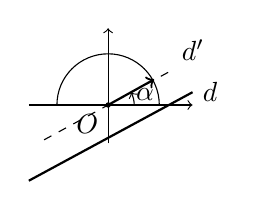
\begin{tikzpicture}[scale=0.65]
  \draw[->] (-1.55,0)--(1.65,0);
  \draw[->] (0,-0.75)--(0,1.50);
  \draw (-1,0) arc[start angle=180,end angle=0,radius=1];
  \draw[thick] (-1.55,-1.48)--(1.65,0.25) node[right] {$d$};
  \draw[dashed] (-1.25,-0.68)--(1.25,0.68) node[above right] {$d'$};
  \draw[->,thick] (0,0)--(0.9,0.5);
  \draw[->] (0.51,0) arc[start angle=0,end angle=29,radius=0.51];
  \node at (0.72,0.20) {$\alpha$};
  \fill (0,0) circle (1.5pt) node[below left] {$O$};
\end{tikzpicture}
\end{center}

\[
\begin{tikzcd}[column sep=large,row sep=large]
 \mathcal D\arrow[r,"p"]\arrow[d,"f"']
   & \mathcal D/{\sim}\arrow[dl,dashed,"\overline f"]\\
 B^1 &
\end{tikzcd}
\]
$f(d)$ este intersecția cu $B^1$ a dreptei paralele cu $d$
care trece prin $O$.
În notițe:
\[
 R_f=\sim,\qquad f\text{ este surjectivă},
\]
și rezultă existența unei aplicații induse bijective
\[
 \exists!\,\overline f:\mathcal D/{\sim}\longrightarrow B^1,
 \qquad \overline f\text{ este bijectivă}.
\]

\medskip
\noindent\textbf{Exercițiul 1.}
Fie $B\subseteq A$ mulțimi și pe $\mathcal P(A)$ relația
\[
 X\sim Y\iff X\cap B=Y\cap B.
\]
Arătați că $\sim$ este relație de echivalență și că
\[
 \mathcal P(A)/{\sim}\ \cong\ \mathcal P(B),
 \qquad X\longmapsto X\cap B.
\]

\noindent\textbf{Exercițiul 2.}
Dacă $|M|=n$, să se calculeze numărul relațiilor de echivalență
care se pot defini pe $M$.

\medskip
\noindent Pentru două mulțimi $A,B$ se definește
\[
 A\sim B\ \overset{\mathrm{def}}{\iff}\
 \exists\,f:A\longrightarrow B\text{ bijectivă}.
\]
Aceasta este o relație de echivalență (echipotență). În notițe,
cardinalul este indicat prin
\[
 \boxed{\widehat A\ \overset{\mathrm{not}}{=}
 \operatorname{card}(A)\ \overset{\mathrm{not}}{=}\ |A|}.
\]

\endgroup
; fără preambul sau pagină nouă.
% NOTE EDITORIALE:
% - Relația de pe mulțimea dreptelor este definită prin egalitate ori
%   lipsa intersecției (drepte paralele distincte). Am păstrat această formă.
% - Simbolul manuscris pentru semicercul superior pare B^1 (ușor neclar).
% - În manuscris, B^1 este definit prin |z|=1 și Im(z)>=0, incluzând astfel
%   atât 1, cât și -1. Însă t în [0,pi) exclude -1, deci aplicația indicată
%   nu este surjectivă pe B^1 cu această definiție. Nu am corectat tacit.
% - Formula f(d) ca "intersecție" a paralelei prin O cu semicercul este
%   ambiguă în cazul dreptei orizontale: acea dreaptă întâlnește ambele
%   capete ale semicercului inclusiv. Convenția de capăt trebuie verificată.
% - Desenul geometric și triunghiul comutativ sunt redesenate în TikZ.
% - Enunțurile exercițiilor 1 și 2 sunt transcrise fără soluții noi.
% - La final, notația pentru cardinalitate apare într-un chenar; este
%   păstrată ca notație a manuscrisului, nu drept construcție formală a
%   unei mulțimi a tuturor mulțimilor echipotente.

\subsection*{Seminar 3 - Pagina 9}
\begingroup
\setlength{\abovedisplayskip}{5pt}
\setlength{\belowdisplayskip}{5pt}
\setlength{\abovedisplayshortskip}{3pt}
\setlength{\belowdisplayshortskip}{3pt}

Fie $\mathcal D$ mulțimea dreptelor din plan. Definim
\[
 d_1\sim d_2\ \overset{\mathrm{def}}{\iff}\
 \begin{cases}
 d_1=d_2,\\[-2pt]
 \text{sau}\\[-2pt]
 d_1\cap d_2=\varnothing.
 \end{cases}
\]
Să se arate că $\sim$ este relație de echivalență pe $\mathcal D$ și că
\[
 \mathcal D/{\sim}\ \cong\ [0,\pi).
\]

\noindent\underline{Demonstrație.}
Manuscrisul consideră aplicația injectivă
\[
 [0,\pi)\longrightarrow B^1,\qquad
 B^1=\{z\in\mathbb C\mid |z|=1,\ \operatorname{Im}(z)\geq 0\},
\]
\[
 t\longmapsto\cos t+i\sin t=e^{it}.
\]

\begin{center}
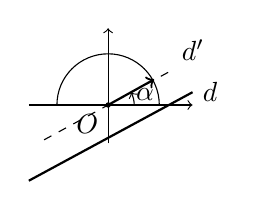
\begin{tikzpicture}[scale=0.65]
  \draw[->] (-1.55,0)--(1.65,0);
  \draw[->] (0,-0.75)--(0,1.50);
  \draw (-1,0) arc[start angle=180,end angle=0,radius=1];
  \draw[thick] (-1.55,-1.48)--(1.65,0.25) node[right] {$d$};
  \draw[dashed] (-1.25,-0.68)--(1.25,0.68) node[above right] {$d'$};
  \draw[->,thick] (0,0)--(0.9,0.5);
  \draw[->] (0.51,0) arc[start angle=0,end angle=29,radius=0.51];
  \node at (0.72,0.20) {$\alpha$};
  \fill (0,0) circle (1.5pt) node[below left] {$O$};
\end{tikzpicture}
\end{center}

\[
\begin{tikzcd}[column sep=large,row sep=large]
 \mathcal D\arrow[r,"p"]\arrow[d,"f"']
   & \mathcal D/{\sim}\arrow[dl,dashed,"\overline f"]\\
 B^1 &
\end{tikzcd}
\]
$f(d)$ este intersecția cu $B^1$ a dreptei paralele cu $d$
care trece prin $O$.
În notițe:
\[
 R_f=\sim,\qquad f\text{ este surjectivă},
\]
și rezultă existența unei aplicații induse bijective
\[
 \exists!\,\overline f:\mathcal D/{\sim}\longrightarrow B^1,
 \qquad \overline f\text{ este bijectivă}.
\]

\medskip
\noindent\textbf{Exercițiul 1.}
Fie $B\subseteq A$ mulțimi și pe $\mathcal P(A)$ relația
\[
 X\sim Y\iff X\cap B=Y\cap B.
\]
Arătați că $\sim$ este relație de echivalență și că
\[
 \mathcal P(A)/{\sim}\ \cong\ \mathcal P(B),
 \qquad X\longmapsto X\cap B.
\]

\noindent\textbf{Exercițiul 2.}
Dacă $|M|=n$, să se calculeze numărul relațiilor de echivalență
care se pot defini pe $M$.

\medskip
\noindent Pentru două mulțimi $A,B$ se definește
\[
 A\sim B\ \overset{\mathrm{def}}{\iff}\
 \exists\,f:A\longrightarrow B\text{ bijectivă}.
\]
Aceasta este o relație de echivalență (echipotență). În notițe,
cardinalul este indicat prin
\[
 \boxed{\widehat A\ \overset{\mathrm{not}}{=}
 \operatorname{card}(A)\ \overset{\mathrm{not}}{=}\ |A|}.
\]

\endgroup
; fără preambul sau pagină nouă.
% NOTE EDITORIALE:
% - Relația de pe mulțimea dreptelor este definită prin egalitate ori
%   lipsa intersecției (drepte paralele distincte). Am păstrat această formă.
% - Simbolul manuscris pentru semicercul superior pare B^1 (ușor neclar).
% - În manuscris, B^1 este definit prin |z|=1 și Im(z)>=0, incluzând astfel
%   atât 1, cât și -1. Însă t în [0,pi) exclude -1, deci aplicația indicată
%   nu este surjectivă pe B^1 cu această definiție. Nu am corectat tacit.
% - Formula f(d) ca "intersecție" a paralelei prin O cu semicercul este
%   ambiguă în cazul dreptei orizontale: acea dreaptă întâlnește ambele
%   capete ale semicercului inclusiv. Convenția de capăt trebuie verificată.
% - Desenul geometric și triunghiul comutativ sunt redesenate în TikZ.
% - Enunțurile exercițiilor 1 și 2 sunt transcrise fără soluții noi.
% - La final, notația pentru cardinalitate apare într-un chenar; este
%   păstrată ca notație a manuscrisului, nu drept construcție formală a
%   unei mulțimi a tuturor mulțimilor echipotente.

\subsection*{Seminar 3 - Pagina 9}
\begingroup
\setlength{\abovedisplayskip}{5pt}
\setlength{\belowdisplayskip}{5pt}
\setlength{\abovedisplayshortskip}{3pt}
\setlength{\belowdisplayshortskip}{3pt}

Fie $\mathcal D$ mulțimea dreptelor din plan. Definim
\[
 d_1\sim d_2\ \overset{\mathrm{def}}{\iff}\
 \begin{cases}
 d_1=d_2,\\[-2pt]
 \text{sau}\\[-2pt]
 d_1\cap d_2=\varnothing.
 \end{cases}
\]
Să se arate că $\sim$ este relație de echivalență pe $\mathcal D$ și că
\[
 \mathcal D/{\sim}\ \cong\ [0,\pi).
\]

\noindent\underline{Demonstrație.}
Manuscrisul consideră aplicația injectivă
\[
 [0,\pi)\longrightarrow B^1,\qquad
 B^1=\{z\in\mathbb C\mid |z|=1,\ \operatorname{Im}(z)\geq 0\},
\]
\[
 t\longmapsto\cos t+i\sin t=e^{it}.
\]

\begin{center}
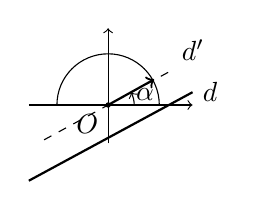
\begin{tikzpicture}[scale=0.65]
  \draw[->] (-1.55,0)--(1.65,0);
  \draw[->] (0,-0.75)--(0,1.50);
  \draw (-1,0) arc[start angle=180,end angle=0,radius=1];
  \draw[thick] (-1.55,-1.48)--(1.65,0.25) node[right] {$d$};
  \draw[dashed] (-1.25,-0.68)--(1.25,0.68) node[above right] {$d'$};
  \draw[->,thick] (0,0)--(0.9,0.5);
  \draw[->] (0.51,0) arc[start angle=0,end angle=29,radius=0.51];
  \node at (0.72,0.20) {$\alpha$};
  \fill (0,0) circle (1.5pt) node[below left] {$O$};
\end{tikzpicture}
\end{center}

\[
\begin{tikzcd}[column sep=large,row sep=large]
 \mathcal D\arrow[r,"p"]\arrow[d,"f"']
   & \mathcal D/{\sim}\arrow[dl,dashed,"\overline f"]\\
 B^1 &
\end{tikzcd}
\]
$f(d)$ este intersecția cu $B^1$ a dreptei paralele cu $d$
care trece prin $O$.
În notițe:
\[
 R_f=\sim,\qquad f\text{ este surjectivă},
\]
și rezultă existența unei aplicații induse bijective
\[
 \exists!\,\overline f:\mathcal D/{\sim}\longrightarrow B^1,
 \qquad \overline f\text{ este bijectivă}.
\]

\medskip
\noindent\textbf{Exercițiul 1.}
Fie $B\subseteq A$ mulțimi și pe $\mathcal P(A)$ relația
\[
 X\sim Y\iff X\cap B=Y\cap B.
\]
Arătați că $\sim$ este relație de echivalență și că
\[
 \mathcal P(A)/{\sim}\ \cong\ \mathcal P(B),
 \qquad X\longmapsto X\cap B.
\]

\noindent\textbf{Exercițiul 2.}
Dacă $|M|=n$, să se calculeze numărul relațiilor de echivalență
care se pot defini pe $M$.

\medskip
\noindent Pentru două mulțimi $A,B$ se definește
\[
 A\sim B\ \overset{\mathrm{def}}{\iff}\
 \exists\,f:A\longrightarrow B\text{ bijectivă}.
\]
Aceasta este o relație de echivalență (echipotență). În notițe,
cardinalul este indicat prin
\[
 \boxed{\widehat A\ \overset{\mathrm{not}}{=}
 \operatorname{card}(A)\ \overset{\mathrm{not}}{=}\ |A|}.
\]

\endgroup
; fără preambul sau pagină nouă.
% NOTE EDITORIALE:
% - Relația de pe mulțimea dreptelor este definită prin egalitate ori
%   lipsa intersecției (drepte paralele distincte). Am păstrat această formă.
% - Simbolul manuscris pentru semicercul superior pare B^1 (ușor neclar).
% - În manuscris, B^1 este definit prin |z|=1 și Im(z)>=0, incluzând astfel
%   atât 1, cât și -1. Însă t în [0,pi) exclude -1, deci aplicația indicată
%   nu este surjectivă pe B^1 cu această definiție. Nu am corectat tacit.
% - Formula f(d) ca "intersecție" a paralelei prin O cu semicercul este
%   ambiguă în cazul dreptei orizontale: acea dreaptă întâlnește ambele
%   capete ale semicercului inclusiv. Convenția de capăt trebuie verificată.
% - Desenul geometric și triunghiul comutativ sunt redesenate în TikZ.
% - Enunțurile exercițiilor 1 și 2 sunt transcrise fără soluții noi.
% - La final, notația pentru cardinalitate apare într-un chenar; este
%   păstrată ca notație a manuscrisului, nu drept construcție formală a
%   unei mulțimi a tuturor mulțimilor echipotente.

\subsection*{Seminar 3 - Pagina 9}
\begingroup
\setlength{\abovedisplayskip}{5pt}
\setlength{\belowdisplayskip}{5pt}
\setlength{\abovedisplayshortskip}{3pt}
\setlength{\belowdisplayshortskip}{3pt}

Fie $\mathcal D$ mulțimea dreptelor din plan. Definim
\[
 d_1\sim d_2\ \overset{\mathrm{def}}{\iff}\
 \begin{cases}
 d_1=d_2,\\[-2pt]
 \text{sau}\\[-2pt]
 d_1\cap d_2=\varnothing.
 \end{cases}
\]
Să se arate că $\sim$ este relație de echivalență pe $\mathcal D$ și că
\[
 \mathcal D/{\sim}\ \cong\ [0,\pi).
\]

\noindent\underline{Demonstrație.}
Manuscrisul consideră aplicația injectivă
\[
 [0,\pi)\longrightarrow B^1,\qquad
 B^1=\{z\in\mathbb C\mid |z|=1,\ \operatorname{Im}(z)\geq 0\},
\]
\[
 t\longmapsto\cos t+i\sin t=e^{it}.
\]

\begin{center}
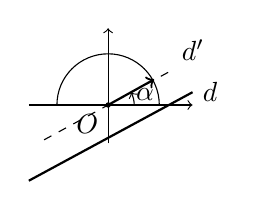
\begin{tikzpicture}[scale=0.65]
  \draw[->] (-1.55,0)--(1.65,0);
  \draw[->] (0,-0.75)--(0,1.50);
  \draw (-1,0) arc[start angle=180,end angle=0,radius=1];
  \draw[thick] (-1.55,-1.48)--(1.65,0.25) node[right] {$d$};
  \draw[dashed] (-1.25,-0.68)--(1.25,0.68) node[above right] {$d'$};
  \draw[->,thick] (0,0)--(0.9,0.5);
  \draw[->] (0.51,0) arc[start angle=0,end angle=29,radius=0.51];
  \node at (0.72,0.20) {$\alpha$};
  \fill (0,0) circle (1.5pt) node[below left] {$O$};
\end{tikzpicture}
\end{center}

\[
\begin{tikzcd}[column sep=large,row sep=large]
 \mathcal D\arrow[r,"p"]\arrow[d,"f"']
   & \mathcal D/{\sim}\arrow[dl,dashed,"\overline f"]\\
 B^1 &
\end{tikzcd}
\]
$f(d)$ este intersecția cu $B^1$ a dreptei paralele cu $d$
care trece prin $O$.
În notițe:
\[
 R_f=\sim,\qquad f\text{ este surjectivă},
\]
și rezultă existența unei aplicații induse bijective
\[
 \exists!\,\overline f:\mathcal D/{\sim}\longrightarrow B^1,
 \qquad \overline f\text{ este bijectivă}.
\]

\medskip
\noindent\textbf{Exercițiul 1.}
Fie $B\subseteq A$ mulțimi și pe $\mathcal P(A)$ relația
\[
 X\sim Y\iff X\cap B=Y\cap B.
\]
Arătați că $\sim$ este relație de echivalență și că
\[
 \mathcal P(A)/{\sim}\ \cong\ \mathcal P(B),
 \qquad X\longmapsto X\cap B.
\]

\noindent\textbf{Exercițiul 2.}
Dacă $|M|=n$, să se calculeze numărul relațiilor de echivalență
care se pot defini pe $M$.

\medskip
\noindent Pentru două mulțimi $A,B$ se definește
\[
 A\sim B\ \overset{\mathrm{def}}{\iff}\
 \exists\,f:A\longrightarrow B\text{ bijectivă}.
\]
Aceasta este o relație de echivalență (echipotență). În notițe,
cardinalul este indicat prin
\[
 \boxed{\widehat A\ \overset{\mathrm{not}}{=}
 \operatorname{card}(A)\ \overset{\mathrm{not}}{=}\ |A|}.
\]

\endgroup
